\section{Bayesian games}
\Que{Bayesian games}
\Ans[Bayesian games]{ are games of incomplete information, where some players do not have complete knowledge on the other players' utility. Bayesian games have the following assumptions:
\begin{itemize}
    \item Each player i has a set of possible types $T_I=\{\text{type 1},...,\}$
    \item The type of each player $t_1,...,t_n$ is determined by Nature's move at the beginning of the game.
    \item Each player knows only his/her type
    \item Other player's type is unknown
\end{itemize}}
\Que{Preliminary Nature's move}
\Ans[]{Bayesian game scan be seen as a weird kind of dynamic games that is played as follows: Nature draws the type vector $(t_1,..,t_n)$ among all the possible combination of players' types; Nature reveals type $t_i$ only to player i; player choose their action; Final payoffs are computed.}
\Que{Beliefs in Bayesian games}
\Ans[]{To find best responses player create beliefs about these types under the assumption that players do not precisely know the types of their opponents but they have an estimate of those. In other words, they know the probability distribution of the opponents' types. This is called the common prior assumption.}
\Que{Bayesian entry game}
\Ans[]{We have an incumbent (player 1) and and outsider (Player 2). The outsider decides whether to enter the market (E) or stay out (O). The incumbent decides whether to accept the outsider (A) or fight (F). The incumbent could be of two types: reasonable or crazy (in the first case it does not like to fight, in the latter it does). The incumbent knows its type, the outsider estimates reasonable/crazy with probabilities (p,1-p).}
\Que{Normal form of Bayesian games}
\Ans[]{The normal form of Bayesian games can be inferred from the extensive form as we did in dynamic games.}
\Que{Strategies in Bayesian games}
\Ans[]{A strategy specifies what the player does for each type. In the entry game: Player one has two strategies $\{O,E\}$, while player 2 has four strategies: $\{AA,AF,FA,FF\}$. For example if 2 plays AF it means play A if reasonable or play F if crazy.}
\Que{Example to understand the normal form:}
\includepdf[pages=16-23,nup=1x2,landscape=false]{Appendix/Lecture18.pdf}
\Que{Bayesian game: definition}
\Ans[]{It is described as follows:
\begin{itemize}
    \item Set of players $\{1,..,n\}$
    \item Strategy sets $S_1,..,S_n$
    \item Utility functions $u_i:\S_1\times ...\times S_n\rightarrow \mathbb{R}$(for i=1,...,n)
    \item \textbf{Type space} of each player $T_i$
    \item \textbf{Type-dependent utilities:} define $u_i(a_1,...,a_n,t_i)$ for each $t_i\in T_i$
    \item \textbf{Beliefs about players types: }a probability distribution $\phi_i$ defined over types for each player
\end{itemize}}
\Que{Static Bayesian game}
\Ans[]{Consider a static Bayesian game: n players, each player's strategy is just an action:
\begin{itemize}
    \item Player i's type is $t_i\in T_i$, chosen by Nature for each player from 1 to n through the joint prior probability distribution $\phi(t_1,...,t_n)$ where $\phi:T_1\times ...\times T_n\rightarrow[0,1]$
    \item Player i knows his private values of his/her utility function $u_i(a_1,...,a_n,t_i)$
\end{itemize}}
\Que{Type of a player}
\Ans[]{Suppose i can have two different payoff functions $u_{i,A}(a_i,a_{-i})$ and $u_{i,B}(a_I,a_{-i})$. We represent this by setting a type space $T_i=\{t_A,t_B\}$ and imposing $u_{i,j}(a_i,a_{-i})=u_i(a_i,a_{-i},t_j)$.\\
Types can be correlated; they are independent if
\[
\phi(t_1,...,t_n)=\phi(t_1)...\phi(t_n)
\]}